\documentclass[12pt]{article}

\usepackage{titlesec}
\usepackage{multirow}
\usepackage{fullpage}
\usepackage{array}
\usepackage{graphicx}

\usepackage{biblatex}
\bibliography{sources.bib}

\newcommand{\sectionbreak}{\clearpage}

\begin{document}
\section{Executive Summary}
3D scanning has a wide variety of applications, but the high cost of these
scanners keeps the technology from being used in many potential applications.
Bringing down the cost and complexity of accurate 3D scanning would enable the
use of 3D scanning in many applications where it now is prohibitively expensive:
research labs, hobbyist builders, 3D printing enthusiasts, artists, independent
product designers, small manufacturers, etc.

We found that there is an academically popular method, structured light
scanning, that maintains high scan accuracy, at lower costs. However, there is
typically a large degree of complexity in setting up a structured light scanner;
streamlining this service and packaging it	 into a plug-and-play device will
enable us to sell the product to markets that currently cannot access or afford
3D scanning. Additionally, we have ways to make the product even less expensive
than typical structured light scanners by substituting inexpensive components,
such as smart phone cameras, in clever ways.

In short, we want to bring 3D scanning to a large group of users who cannot
access it today. We will do this by building a low-cost, user-friendly, and
high-accuracy, 3D scanner.

\section{Market Overview}
Digital 3D scanning is a large, established market, with an estimated market
size of \$530 million.  Most of the products in this market are high-end
and targeted at large corporations, costing tens of thousands of dollars.
Reductions in component costs, advances in algorithmic efficiency, and increases
in computing power now enable inexpensive 3D scanners that can achieve
accuracy levels that are comparable to the expensive units.

Through building an accessible, affordable, desktop 3D scanner, we hope to
expose a new, untapped market. The desktop 3D printing market has been
experiencing rapid growth over the past few years, growing 240\% each year from
2006 to 2011\cite{wohlers}. The primary customers for desktop 3D printers have been
individuals: hobbyists, independent designers, artists, etc. We believe that
this same market segment will buy an inexpensive desktop 3D scanner. In fact, we
believe that 3D scanners will be the standard measurement tool used in shops,
labs and studios. We believe that 3D scanners should be as common as a purchase
as a cordless drill.

The 3D scanner that this market needs requires a set of qualities that we believe no
other scanner on the market currently has:
\begin{itemize}
\item It must be painless to use.  From opening the box, the user needs to be
  able to plug the scanner into his computer, put an object in the scanner,
  press scan, and then have a 3D model appear on his computer.
\item It must be affordable.  The scanner cannot cost so much that it is a
  luxury to the user.  We judge that the scanner must be in the \$300-\$600
  price range.
\item It must be useful.  The scanner needs to have an accuracy high enough to
  not be a constraint on most machining processes or 3D printing processes.  It
  cannot take too long to scan. It must be able to scan all objects that can be
  3D printed, and a significant percentage of objects that would be used in a design.
\end{itemize}

The market segment we are targeting be divided into individual consumers and small
(< 10 people) enterprises.

The individual consumers we are targeting are hobbyists, enthusiasts, and
artists. Many people have become excited about desktop 3D printing, and will be
similarly excited by desktop 3D scanning. There is evidence for this recent
successful crowd-sourced fundings for desktop 3D scanning projects, and
excitement surrounding 3D scanning announcements. Though much of the popular
focus has been on scanning objects in order to get a model to print, other uses
of 3D scanners can be marketed. A sculptor may want to display his work online,
or send an early version of a sculpture to a colleague; our scanner allows him
to do so with ease. A garage tinkerer may need to get the dimensions of an
object he wants to incorporate into a larger project. 

The small enterprises we are focusing on include research labs, product
designers, and small machine shops. In research labs, it is often important to
have models and measurements of objects being tested; while the 3D scanners
available today would be an unaffordable luxury, ours would be low-cost enough
to have a practical purpose. Product designers can make initial designs with
physical materials, which are nicer to work with, and then scan them to get a
usable CAD model. Small manufacturers and machine shops can use them in the same
fashion that large manufacturers do: for automated verification of manufactured
parts, as well as for designing parts with unknown dimensions.

As 3D scanning technology has existed for a good deal of time, there are 

Our competitors can be separated into 3 categories:

The current lowest-cost high-accuracy options: The major competitors in this
range would be the NextEngine scanner or Artec's 3D scanners. Our price (~\$500)
will be significantly lower than these products, and our scanner will be easier
to use than the NextEnginer scanner. The NextEngine costs over \$3,000 (once
you've purchased all the necessary software), and the least expensive Artec
scanner costs \$12,000. Our scanner's accuracy will be in the same range as
these products. Unlike these products, however, our scanner will only be able to
scan objects that are under a certain size. While the Artec scanners make
scanning large objects fairly simple, scanning large objects with the NextEngine
is very inconvenient, which is also true for other products in the their range.

The very low-cost (free) options: There are some options on the market that come
in at a price lower than ours. AutoDesk as an free app called 123D Catch--you
take a series of images of an object and then it performs image reconstruction
to generate a 3D model. Some products (like Scanect) allow a customer to use a
Kinect to perform 3D scanning, and Microsoft recently released KinectFusion,
which turns the Kinect into a 3D scanner for anyone with the Windows Kinect SDK.
These technologies, though, do not provide the level of accuracy we are seeking,
or the ease of access. They have more difficulty with highly specular objects
than we will, and require user participation during the entire scanning process.

The emerging competitors: There are a couple competitors that have announced
products but don't have anything for sale yet. CADScan successfully completed a
Kickstarter project for a desktop 3D scanner that will be similar to ours in
terms of target specifications and customers. From the Kickstarter funding
levels, it seems that they plan on charging at least £650 (\$1000) for the
scanner, a price we are planning to come in significantly below. MakerBot also
just announced at SXSW that they will be producing a desktop 3D scanner called
the Digitizer. The announcement was very nebulous on details, but given their 3D
printer costs and their description of the Digitizer, we surmise that they will
be charging over \$1500.


\section{Innovation and Approach}
Approach of our venture including its unique technology approaches/ideas:

There are already many well developed techniques for 3D scanning, so rather than
reinvent the wheel the team spent a week researching 12 techniques and assessing
each for their relevance and compatibility for our product�s goals. We concluded
that �structured light� scanning, a basic triangulation method, would be the
simplest and cheapest to execute.

From wikipedia�s article on �Structured Light�:

Structured light is the process of projecting a known pattern of pixels (often
grids or horizontal bars) on to a scene. The way that these deform when striking
surfaces allows vision systems to calculate the depth and surface information of
the objects in the scene, as used in structured light 3D scanners.

There are tutorials online for how consumers can set up their own structured
light scanners using a standard projector and a digital camera, but the amount
of time required to calibrate the scanner and the hardware required makes the
do-it-yourself approach both prohibitively difficult and expensive.
Off-the-shelf already calibrated units are in the \$3000 range and still don�t
boast the type of resolution that structured-light scanning techniques are
accurate to.

What we require for our product (a pre-calibrated, affordable, high-resolution
3D scanner) is a [1] projection system, [2] an imaging system, and [3] the
software to process the acquired data and generate a point cloud. The following
discusses our development of the three subsystems so far.

[1] Projection:

In order to get around the requirement of having a standard projector (for which
the cheapest units retail for \$300 in the US, \$75 from China) we instead
looked into the cheapest way that we could project a static, high-contrast image
on our object. We looked into doing this using the interference properties of
coherent laser light but instead opted for projecting a high contrast silhouette
of a grating onto the object. Using simple geometric arguments, the factor
limiting the contrast of the projected silhouette is simply the size of the
light source (as one can imagine, the projected image is simply the image
created by a point light source convolved over the size of the light source).
Our approach: to focus a well-collimated light source down to a single point �-
effectively creating a point light source �� and then allowing it to propagate
through the focal point and diverge to cover an area large enough to cover our
whole object. All that this requires is a single lens and a collimated light
source, for which we used a laser and a 15mm focal length lens from Thorlabs,
but from initial testing we believe we can improve on the existing setup
substantially while still keeping costs low. Employing a well-collimated,
incoherent, white light source and a system of lenses should allow us to get rid
of unwanted interference patterns and project a large enough image from less
than 2 feet away.

[2] Imaging:

The Smartphone industry has helped create a large demand for small, high
resolution, inexpensive imaging sensor. These imaging sensors are the bare bones
of digital cameras for only a fraction of the cost. The sensors are available
for less than \$10 ,even in small quantities, and can produce images in the 5-8
megapixel range. The imaging sensors allow us to maintain affordability while
still provide high accuracy. Microcontrollers are also at a point where they are
cheap, but easily powerful enough to utilize the full potential of the sensor.
Craig is currently doing development using a Cypress PSoC (Programmable System
on Chip), which allows for fast prototyping, without the need for peripheral
chips, as they can be programmed into the PSoC. This minimizes downtime wiring
chips or designing Printed Circuit Boards, and reduces cost.

[3] Software:

\section{Lessons Learned}

Imaging:
Many of the issues that arose from prototyping have to do with the physical layout of the circuits. Many of the advanced sensors come in a format that is difficult to work with. The chips come in a Ball Grid Array package, which is not easily dealt with by prototyping. The grid consists of 56 balls of solder each spaced about 500-600$\mu$m apart, which are impossible to solder to directly; they must be reflowed onto a PCB. While this should not be a problem when dealing with the end product, it means that developmental tools are invaluable during initial phases. 

\section{Plan of Action}
Following are the actions we will plan on completing, with more emphasis on
tasks to complete over the summer.

\subsection{Customer Milestones}
\begin{table}[h!]
\begin{tabular}{|p{4.5in}|c|}
\hline
Milestone & Date \\ \hline
Estimate consumer market demand via a Google Consumer Survey (or equivalent
technique) & 6/20 \\
Choose product name and create logo as a reflection of desired brand image &
8/1 \\ 
Secure list of prototype testing partners & 8/15 \\ 
\hline
\end{tabular}
\end{table}

\subsection{Product Milestones}
\begin{table}[h!]
\begin{tabular}{|p{4.5in}|c|}
\hline
Milestone & Date \\ \hline
Finalize the low-cost projection method that will be used in the system & 7/1 \\
Develop an IP strategy to protect crucial design components of the system, and
file for provisional patents is appropriate & 7/15 \\
Complete alpha prototype of the system & 9/1 \\ 
Complete $2^{nd}$ alpha prototype of the system & 10/1 \\ 
Develop a list of components for a beta prototype, and select manufacturing
partners to source parts from  & 11/1 \\ 
Complete beta prototype & 12/1 \\
\hline
\end{tabular}
\end{table}

\subsection{Team Milestones}
\begin{table}[h!]
\begin{tabular}{|p{4.5in}|c|}
\hline
Milestone & Date \\ \hline
Finalize team members' equity splits and vesting schedules, defining 
what will happen under different possible participation scenarios. & 6/15 \\
Bring in an additional team member with business experience to aid in business
strategy, scaling, and marketing & 9/1 \\
\hline
\end{tabular}
\end{table}

\subsection{Financial Milestones}
\begin{table}[h!]
\begin{tabular}{|p{4.5in}|c|}
\hline
Milestone & Date \\ \hline
Develop a high quality short and long pitch deck & 7/1 \\
1st order estimate of unit manufacturing costs at various build volumes using
alpha prototype components & 8/15 \\
Secure funding in order to continue growing the business & 9/1 \\
\hline
\end{tabular}
\end{table}

\section{Risk Factors}

\begin{tabular}[b]{|p{3cm} | p{5cm}| p{2cm}| p{5cm}|}
\hline 

Risk Catergory & \centering{Risk} & \centering{Probability of Risk \newline Materializing}& Risk Mitigation \\ 
\hline
\multirow{2}{*}{Management Team}
& Having only  technically oriented cofounders could leave us weak in terms of business strategy and entrepreneurial prowess&\centering{High} & We must recruit another employee or cofounder who is business and marketing oriented \\  \cline{2-4} 
&Team unable to strategize operational plans to guide all steps of value chain & \centering{Medium}& Proactively seek advice from experienced advisors and industry experts; implement monitoring and quality checks on a scheduled basis \\  \hline



\multirow{4}{*}{Market} 
&Over or under-estimated market size segmentation and location, such that operational and financial impact will be high & \centering{Medium} & Target a statistically-rationalized need based audience. Perform a more thorough market analysis prior to product launch and design for operational flexibility to meet changes in demand\\ \cline{2-4}
& Inability to capture targeted market, leading to lower sales than anticipated  &\centering{Medium} & Run an aggressive advertising campaign to attract new users. Verify that product aspects appeal to user-base by performing comprehensive usability tests \\ \cline{2-4}
& Unexpected competition penetrates target market &\centering{ Low} & Focus on getting the product to market as quickly as possible. Track market trends and rising competition; design flexible and adaptable strategy to account for requirements to change aspects of product differentiation to stand apart \\ \cline{2-4}
& Technical gap between potential customers and product use requirements hinders sales & \centering{Dramatically High}& It is essential that the product be "plug-and-play". We must balance giving the user adequate control over the settings, while at the same time make sure that the scanner can be run by someone with minimal experience\\ \hline
\end{tabular}

\newpage

\begin{tabular}[b]{|p{3cm} | p{5cm}| p{2cm}| p{5cm}|}
\hline 
\multirow{3}{*}{Finance} 
& Unable to secure adequate funds for prototyping and scale-up & \centering{High} &  Apply for accelerators, VC's and Angels. A working prototype will dramatic help in this regard \\ \cline{2-4}
& Lack of adequate funds to fairly compensate desired talent & \centering{Low} & Ensure that realistic and competitive salaries and benefits are included in all financial models \\ \cline{2-4}
& Unmet supply and demand projections will lead to unbalanced revenues with fixed and variable costs, such that unit price exceeds initial estimate. This will lower market absorption and increase time to break-even & \centering{Medium} & Identify the largest sources of cost and strategize how to best mitigate. Alternatively, depending on the market, we might find that our current target price point can be increased without severely impacting sales \\ \hline

Delivery& Difficulties with shipping and packaging  & \centering{Low}& Connect with experienced mentors or consultants, and keep delivery channels in mind during design \\ \hline
\end{tabular}

\section{Team}
*Troy's Bio Troy is graduating this June with majors in 16-ENG (concentration in
Robotics) and 8B (concentration in Computational Learning Systems), and a minor
in 14. The majority of his experience is as a programmer, focusing on machine
learning and web development. He plays tennis for MIT and is a Freshman
Leadership Program counselor.

\textbf{Craig} is pursuing his degree in 2A-6, Mechanical Engineering with a
concentration in Control, Instrumentation and Robotics. He has worked
extensively with robotics and machine design since freshman year of high school. This past semester his team won the 2.12, Introduction to Robotics, term Robo-Gymnastics competition. The team won their division, the overall competition, and was awarded ``Best Design Award''. Additionally, Craig was awarded ``Most Valuable Engineer'' for his team. In addition to mechanical engineering, Craig is experienced with microcontrollers, software and embedded systems. Craig is currently president of
his fraternity, captain of the varsity Waterpolo team, and a member of the
national varsity swim team.

*Gus's Bio Gus is receiving his BS in physics from MIT this June. His focus has
been on ultra-cold atomic physics, and he has worked in 5 different labs ranging
from condensed matter physics to plasma physics. He sings with the Logarhythms,
is a Freshman Leadership Program counselor, is a (half) Iron Man, and cooks a
mean pork roulade.

* How long have you known each other, and what have you worked on in the past?
(Include past work done on this project, if applicable.) We have been working on
this project together since January, as part of 6.S078, Entrepreneurship
Project. We have been working with another student as well, Turner Bohlen.
Unfortunately Turner won't be able to join us for the summer as he has previous
commitments.

Troy and Gus have known each other since their freshman year, and have been
co-counselors in the Freshman Leadership Program for the past 2 years. Craig and
Troy took the same robotics class, 2.12 Intro to Robotics, in the Fall of 2012
where they both placed in the top 5 out of 70 students.

\section{Financial Plan}

\textbf{Annual Growth Rate}(to year 3): 2.4
\newline
\textbf{Quarterly}: 0.3579
\newline
\textbf{Initial Annual Sales} :4000 units
\newline
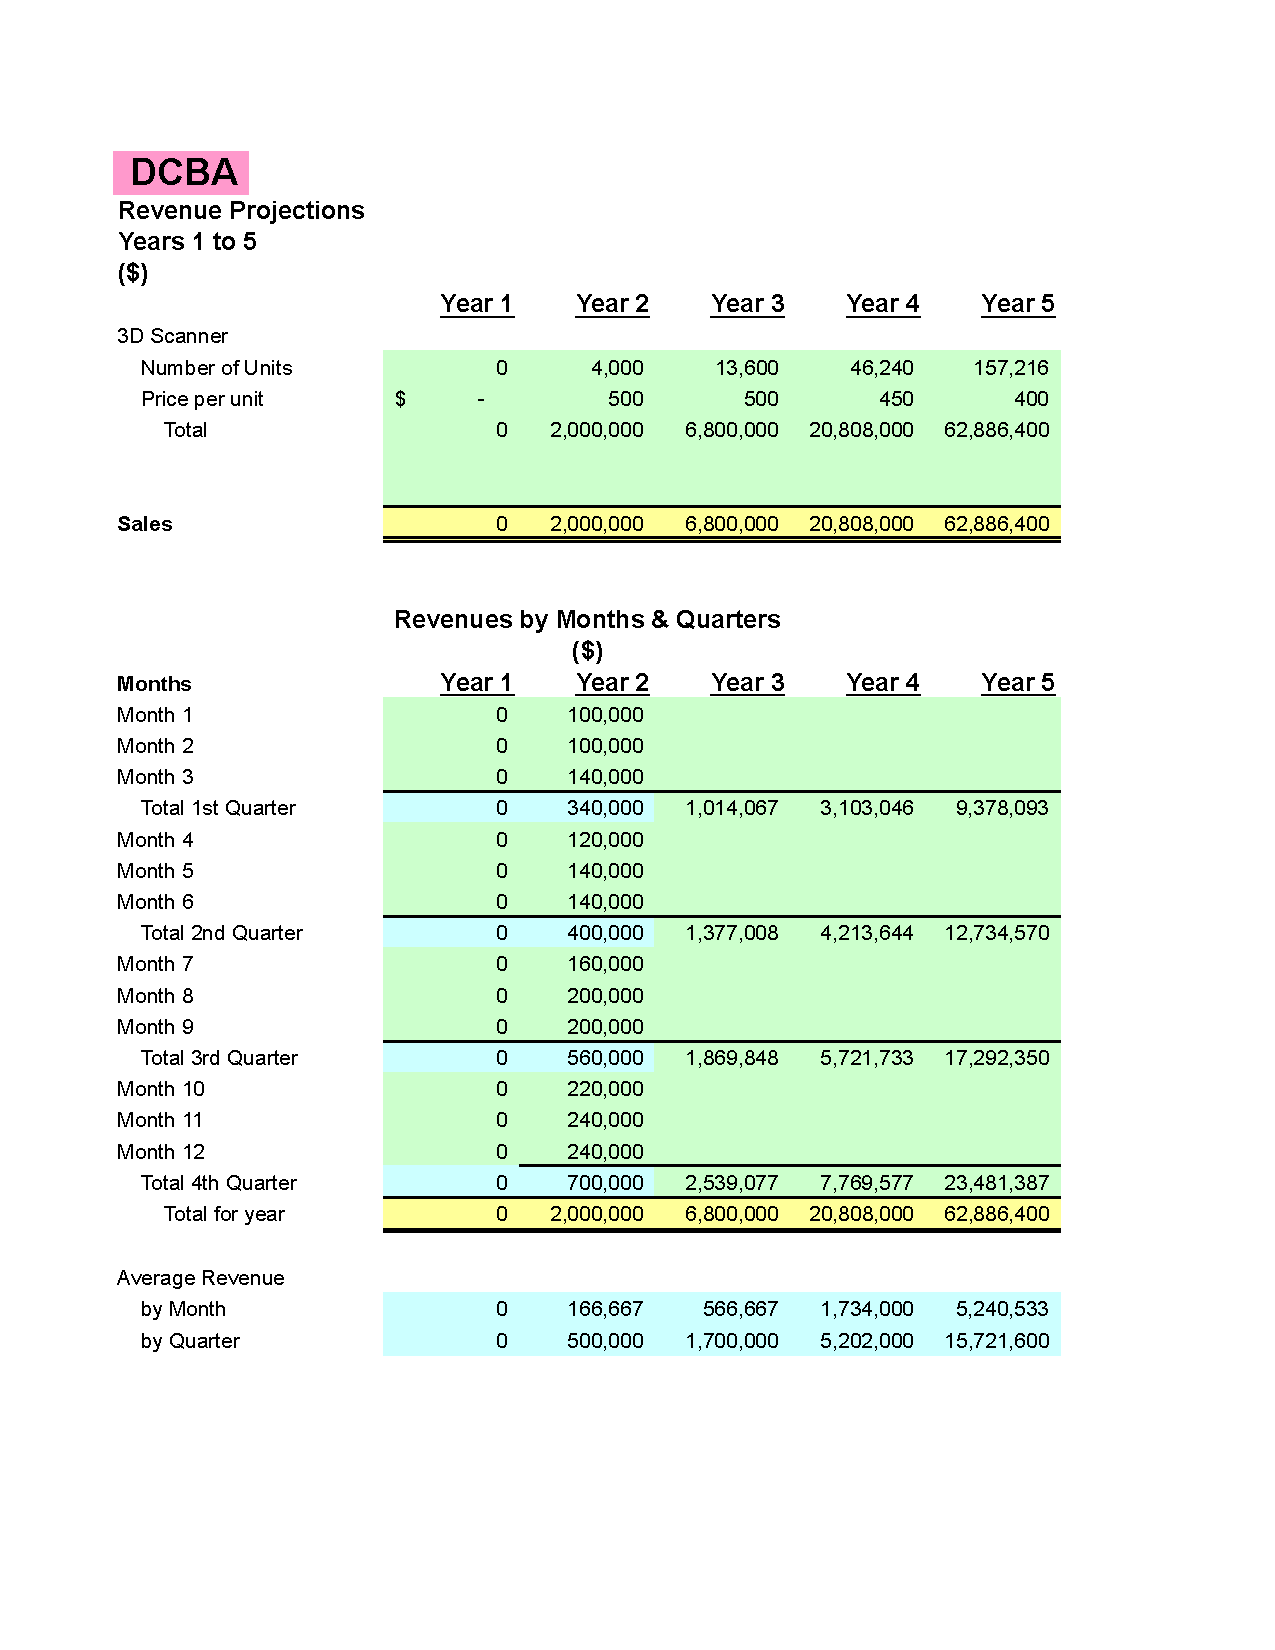
\includegraphics[scale=.75]{finance02.pdf}
\newpage
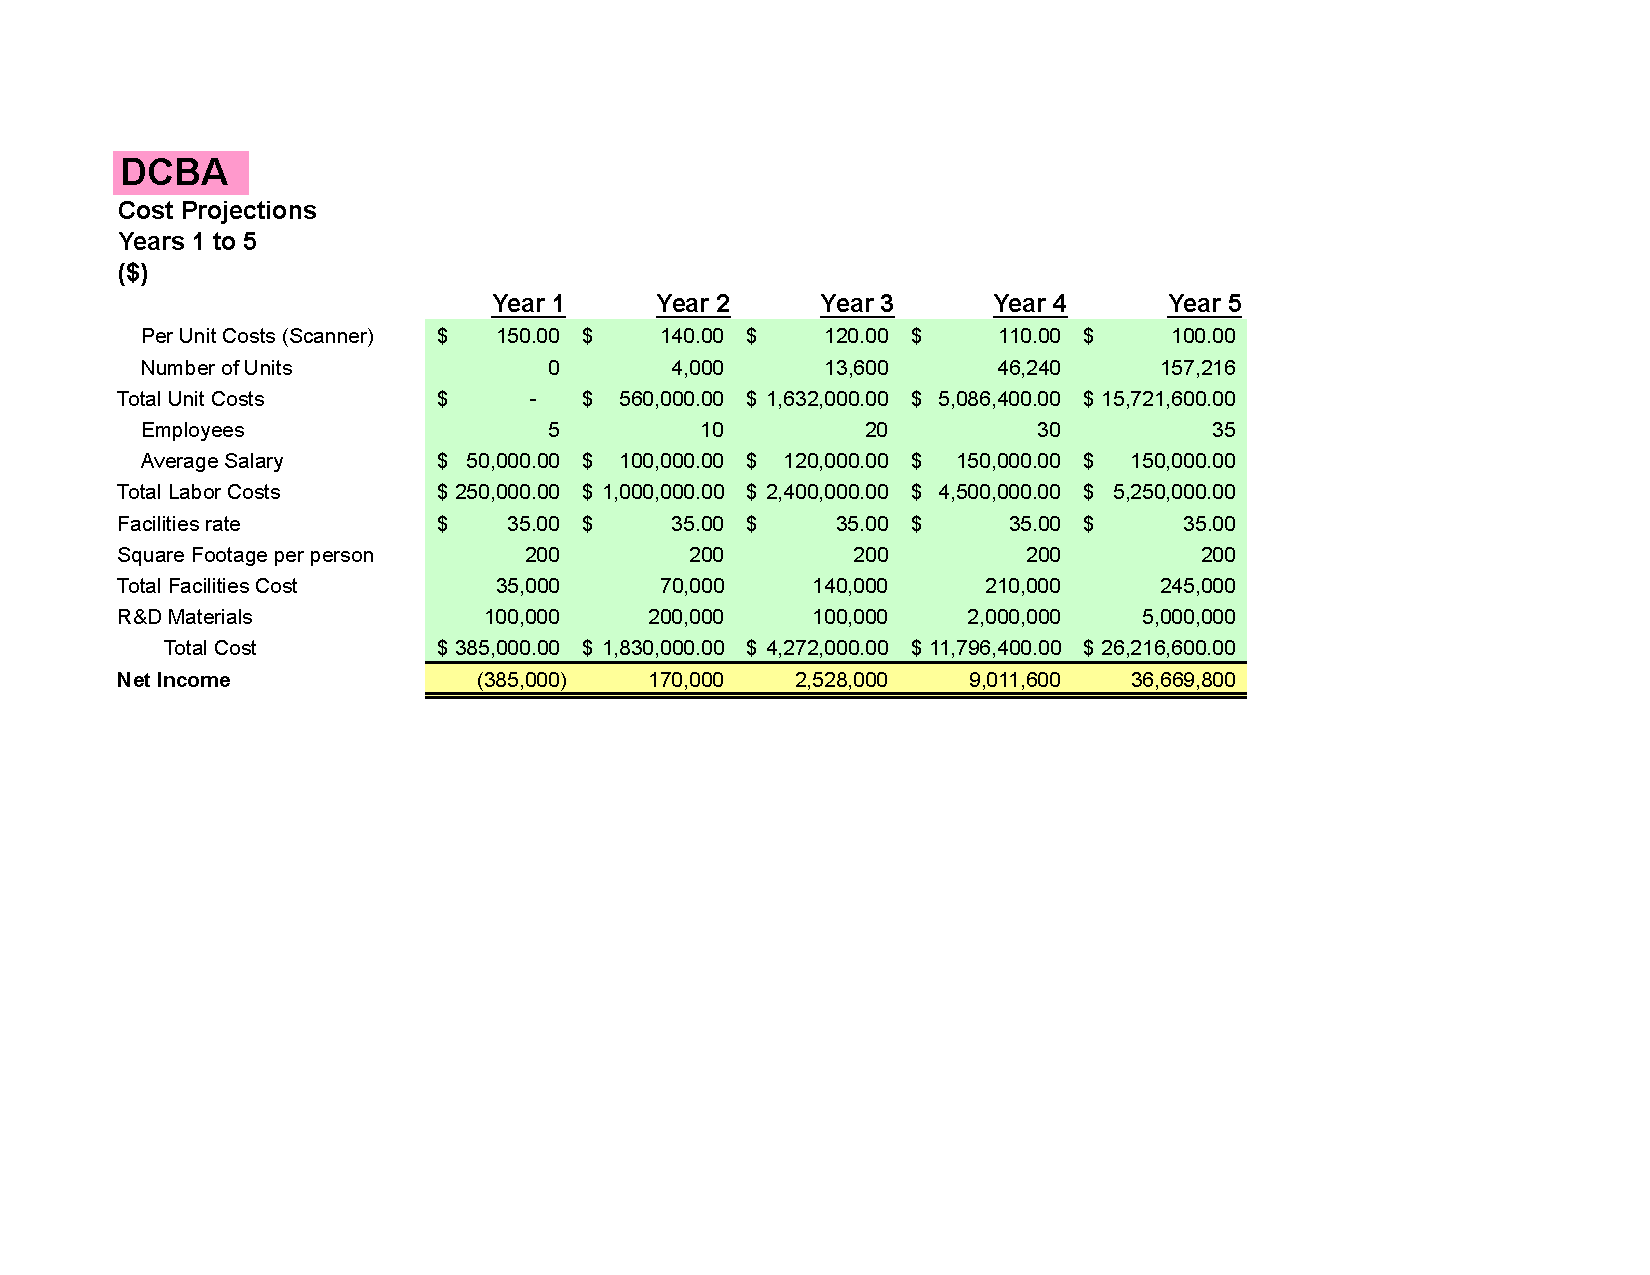
\includegraphics[scale=.75]{finance01.pdf}

\nocite{*}
\printbibliography

\end{document}
